%\documentstyle[epsf,twocolumn]{jarticle}       %LaTeX2e仕様
\documentclass[twocolumn]{jarticle}     %pLaTeX2e仕様(platex.exeの場合)
%\documentclass[twocolumn]{ujarticle}     %pLaTeX2e仕様(uplatex.exeの場合)
%%%%%%%%%%%%%%%%%%%%%%%%%%%%%%%%%%%%%%%%%%%%%%%%%%%%%%%%%%%%%%
%%
%%  基本バージョン
%%
%%%%%%%%%%%%%%%%%%%%%%%%%%%%%%%%%%%%%%%%%%%%%%%%%%%%%%%%%%%%%%%%
\setlength{\topmargin}{-45pt}
%\setlength{\oddsidemargin}{0cm} 
\setlength{\oddsidemargin}{-7.5mm}
%\setlength{\evensidemargin}{0cm} 
\setlength{\textheight}{24.1cm}
%setlength{\textheight}{25cm} 
\setlength{\textwidth}{17.4cm}
%\setlength{\textwidth}{172mm} 
\setlength{\columnsep}{11mm}

\kanjiskip=.07zw plus.5pt minus.5pt


% 【節が変わるごとに (1.1)(1.2) … (2.1)(2.2) と数式番号をつけるとき】
%\makeatletter
%\renewcommand{\theequation}{%
%\thesection.\arabic{equation}} %\@addtoreset{equation}{section}
%\makeatother

%\renewcommand{\arraystretch}{0.95} 行間の設定

%%%%%%%%%%%%%%%%%%%%%%%%%%%%%%%%%%%%%%%%%%%%%%%%%%%%%%%%
\usepackage[dvipdfmx]{graphicx}   %pLaTeX2e仕様(\documentstyle ->\documentclass)\documentclass[dvipdfmx]{graphicx}
\usepackage[dvipdfmx]{color}
\usepackage[subrefformat=parens]{subcaption}
\usepackage{colortbl}
\usepackage{multicol}
%%%%%%%%%%%%%%%%%%%%%%%%%%%%%%%%%%%%%%%%%%%%%%%%%%%%%%%%

\begin{document}

\twocolumn[
\noindent

\hspace{1em}
2021年01月15日
\hfill
\ \ 細川 岳大

\vspace{2mm}

\hrule

\begin{center}
{\Large \bf 進捗報告}
\end{center}
\hrule
\vspace{3mm}
]

% ‚ここから 文章 Start!

\section{今週やったこと}

\begin{itemize}
	\item GAの実験
\end{itemize}

\section{FixMatch の変換操作の探索}
\subsection{設定}
画像変換は\{AutoContrast, Brightness, Color, Contrast, Equalize, Identity, Posterize, Rotate, Sharpness, ShearX/Y, Solarize, TranslateX/Y\}の14種(一つは恒等変換)を用い,各遺伝子はその遺伝子座に対する変換を RandAugment に用いるかいなかについて0/1の値を持つビットエンコーディングとした.また,\ FixMatch\ における弱及び強変換に対し持つので遺伝子長は28とした.

選択はサイズ2のトーナメント選択,交叉には一様交叉,突然変異は遺伝子座ごとに対立遺伝子に置換されるように設定した.

表\ref{tb:GApara1},\ref{tb:FTXpara1}に実験の設定を示す.

\begin{table}[h]
	\centering
	\caption{実験1のGAの設定\label{tb:GApara1}}
	\scalebox{1.0}{
		\begin{tabular}{|c||c|} \hline
			個体数&40\\ \hline
			交叉率&1.0\\ \hline
			突然変異率&0.03\\ \hline
		\end{tabular}
	}
\end{table}

\begin{table}[h]
	\centering
	\caption{実験1の設定\label{tb:FTXpara1}}
	\scalebox{1.0}{
		\begin{tabular}{|c|c|c|} \hline
			model&\multicolumn{2}{c|}{WideResNet16-2}\\ \hline\hline
			data set&\multicolumn{2}{c|}{cifar10}\\ \hline
			train&labeled&50\\ \cline{2-3}
			&unlabeled&49750\\ \hline
			valid&\multicolumn{2}{|c|}{200}\\ \hline
			test&\multicolumn{2}{|c|}{10000}\\ \hline\hline
			\multicolumn{3}{|c|}{事前学習}\\ \hline
			batch size&labeled&32\\ \cline{2-3}
			&unlabeled&$32*7$\\ \hline
			augment&labeled&RandAugment\\ \cline{2-3}
			&weak&Identity\\ \cline{2-3}
			&strong&Identity\\ \hline
			optimizer&\multicolumn{2}{c|}{SGD(lr=0.05,momntum=0.9)}\\ \hline
			num\_iterations&\multicolumn{2}{c|}{5000}\\ \hline\hline
			\multicolumn{3}{|c|}{GAの評価}\\ \hline
			batch size&labeled&16\\ \cline{2-3}
			&unlabeled&$16$\\ \hline
			augment&labeled&RandAugment\\ \hline
			num\_iterations&\multicolumn{2}{c|}{3000}\\ \hline
		\end{tabular}
	}
\end{table}

また得られた個体について最終世代における上位10個体を用いて学習した.
\subsection{結果}
図\ref{fig:ex1_1}に適応度の推移を,
図\ref{fig:ex1_2}最終個体における各\ transform\ の累積を示す.

また表\ref{tb:test}テストに対する識別率を示す.
前回と同様探索されたものは過学習を起こし,従来の RandAugment を超えることはできなかった.
変換操作の種類が従来のもので14種なのに対し,探索されたものは平均5種類程度であり訓練させる画像の多様性が非常に少ないものとなってしまっていることが原因であると考えらるが,バグでないか再度調査が必要な気がする.
また,今回は個体数が大きくしたためか前回に比べ収束は少ない.一方で,前回よく選ばれていた AutoContrast が少ないといったことがみられる.

\begin{table}[h]
	\centering
	\caption{テスト識別率\label{tb:test}}
	\scalebox{1.0}{
		\begin{tabular}{|c|c|c|} \hline
			iteration&従来&探索個体\\ \hline
			5000&0.268&0.357\\ \hline
			10000&0.460&0.287\\ \hline
		\end{tabular}
	}
\end{table}

\begin{figure}[h]
	\begin{center}
		\vspace*{3mm}
		\hspace*{-12mm}
		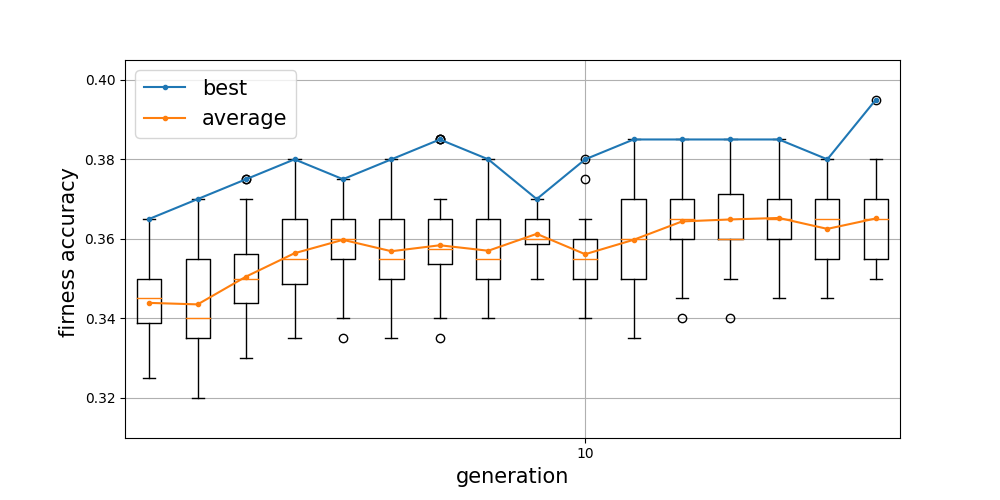
\includegraphics[height=65mm,width=90mm]{graph1_1.png}
		\caption{適応度の推移\label{fig:ex1_1}}
	\end{center}
\end{figure}

\begin{figure}[h]
	\begin{center}
		\vspace*{3mm}
		\hspace*{-12mm}
		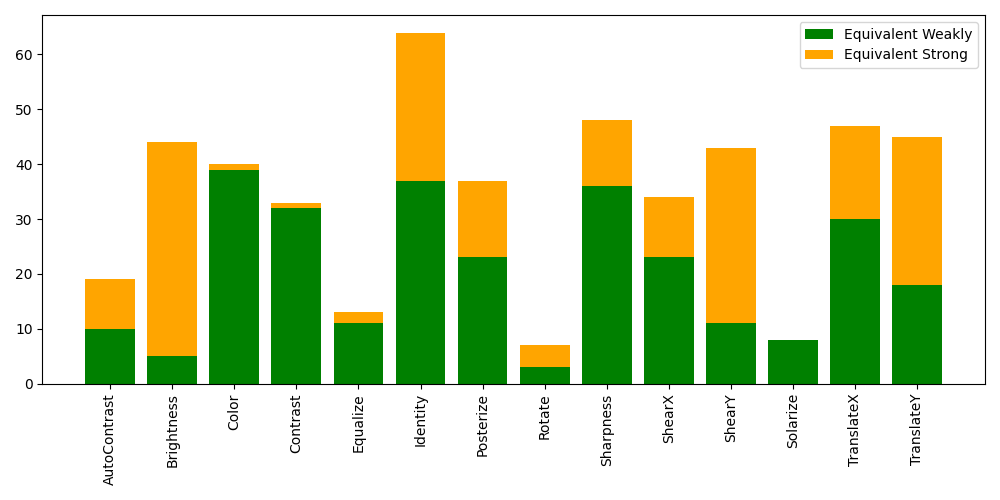
\includegraphics[height=60mm,width=90mm]{graph1_2.png}
		\caption{最終個体\label{fig:ex1_2}}
	\end{center}
\end{figure}

\section{Contrastive Learning の実験}
\subsection{設定}
Contrastive Learning の実装及びGAをからめた実験をした.
個体について,遺伝子は0-9までの整数値のラベルをもち,searchする枚数である50が遺伝子長である.
選択はトーナメント選択(k=3),交叉は2点交叉,突然変異はランダムな別の値に置換するものとした.
表に事前学習の設定を,表\ref{tb:GApara2},\ref{tb:CL2}に設定を示す.

\begin{table}[t]
	\centering
	\caption{実験2のGAの設定\label{tb:GApara2}}
	\scalebox{1.0}{
		\begin{tabular}{|c||c|} \hline
			個体数&40\\ \hline
			交叉率&1.0\\ \hline
			突然変異率&0.1\\ \hline
		\end{tabular}
	}
\end{table}

\begin{table}[h]
	\centering
	\caption{実験2の設定\label{tb:CL2}}
	\scalebox{1.0}{
		\begin{tabular}{|c|c|c|} \hline
			model&Encoder&WideResNet50\\ \cline{2-3}
			&Projection head&2層MLP(shape:2048to512)\\ \cline{2-3}
			&classifer&MLP(shape:2048to10)\\ \hline
			data set&\multicolumn{2}{c|}{cifar10}\\ \hline
			train&labeled&250\\ \cline{2-3}
			&unlabeled&49700\\ \cline{2-3}
			&serach&50\\ \hline
			%test&\multicolumn{2}{|c|}{10000}\\ \hline\hline
			\multicolumn{3}{|c|}{事前学習}\\ \hline
			batch size&\multicolumn{2}{|c|}{64}\\ \hline
			optimizer&\multicolumn{2}{c|}{Adam(lr=$1.0*10^{-3}$,momntum=$1.0*10^{-6}$)}\\ \hline
			epochs&\multicolumn{2}{c|}{75}\\ \hline\hline
			\multicolumn{3}{|c|}{GAの評価}\\ \hline
			batch size&\multicolumn{2}{|c|}{16}\\ \hline
			loss&\multicolumn{2}{|c|}{Cross Entropy Loss}\\ \hline
			optimizer&\multicolumn{2}{c|}{Adam(lr=$5.0*10^{-4}$,momntum=$1.0*10^{-6}$)}\\ \hline
			epochs&\multicolumn{2}{c|}{25}\\ \hline
			valid&\multicolumn{2}{c|}{250(:labeled)}\\ \hline
		\end{tabular}
	}
\end{table}

\subsection{結果}
時間がなかったため表などはありません.
全て正解ラベルを入れた時,識別率が60\%で,
最終世代の最良個体は識別率47.2\%でラベルの正答率は42\%であった.
これまでの探索と同様に正解ラベルではないもので識別率を上げることがあり
やはり GA でラベルを探索することは難しいといえる.一方で,ランダムなラベルからここまでの正答率を出せたのは,
一個体の学習速度が短く世代あたりの個体数を確保できたからだと考えられる.また,今回の実験では元論文に比べ
 Encoder の事前学習は十分でないといえ,また初期個体が今回ランダムであるため,
もう一度実験を行う予定である.

\section{RandAugmentにschedulerを導入した}
\subsection{設定}
GA の画像変換手法の探索において探索されたものが iteration が少ない範囲で識別率がよかったことから
DataAugment でカリキュラム学習のようなことができないかと考えた.

従来の RandAugment は各変換に対し最大最小が決められており,その範囲で強度が一様分布になっている.
今回は強度の分布$Y$について次のように設定することとした.
\begin{eqnarray}
Y=\left\{ \begin{array}{ll}
(1 - 2t)x + t & (-1 \leq x \leq 0) \\
-(1 - 2t)x + t & (0 \leq x \leq 1) \\
0 & (上記以外) \\
\end{array} \right.\\
0 \leq t \leq 1
\end{eqnarray}
$t$を学習のイテレーション数に応じて変化させた.
現在のイテレーション数の最大イテレーション数に対する割合を$iter$としたとき,
以下のものを用意した
\begin{itemize}
	\item $t = a$     ($a$は定数,$a = 0.5$で一様分布)
	\item $t = iter$     (linear)
	\item $t = tanh(4iter - 2)/2 + 0.5$     (tanh)
	\item $t = (2iter - 1)^3 + 0.5$     (cube)
\end{itemize}

\subsection{結果}
図\ref{fig:ex3_1},\ref{fig:ex3_2}に結果を示す.
\begin{figure}[h]
	\begin{center}
		\vspace*{3mm}
		\hspace*{-12mm}
		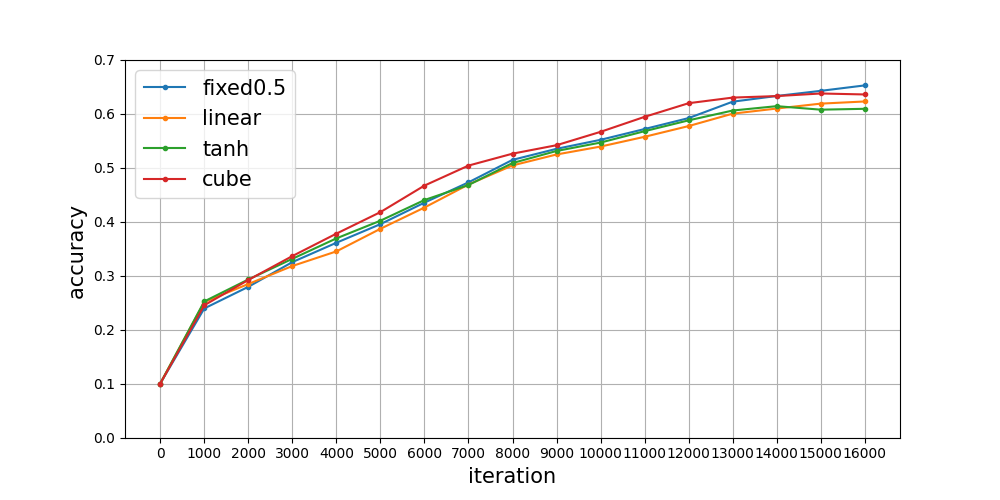
\includegraphics[height=65mm,width=90mm]{acc_1.png}
		\caption{test\_accuracy\label{fig:ex3_1}}
	\end{center}
\end{figure}

\begin{figure}[h]
	\begin{center}
		\vspace*{3mm}
		\hspace*{-12mm}
		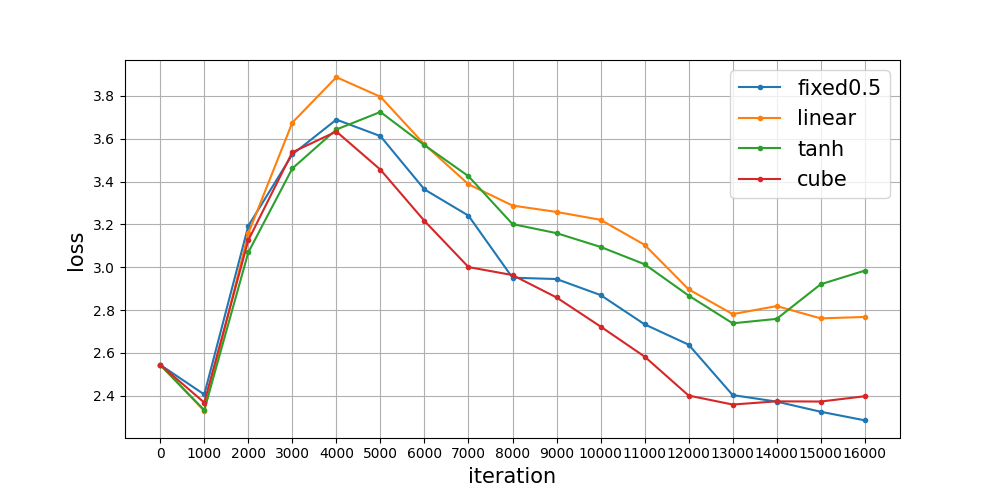
\includegraphics[height=60mm,width=90mm]{loss_1.png}
		\caption{test\_loss\label{fig:ex3_2}}
	\end{center}
\end{figure}

最終的には従来のものに抜かされてはいるものの,cube は他のものよりも少し速い学習が行われていたと言えそうだ.
またこのことから学習最初期に限った話では FixMatch の強変換は強度の低いものがよいと考えられ,GA における探索で時間上イテレーション数が小さくしていたため,それゆえの前回の結果だったと思われる.

\section{来週の課題}
\begin{itemize}
	\item 実験設定の改良
	\item SimCLRを用いた実験
\end{itemize}

\end{document}


